
\section{Running the flagger}

\htmladdnormallink{These slides}{http://www.aoc.nrao.edu/~rurvashi/DataFiles/Talk_FlaggingCASA3.4.pdf}
summarize the CASA flagger infrastructure and user-options.

\htmladdnormallink{Task Documentation}{http://casa.nrao.edu/docs/TaskRef/TaskRef.html}
\htmladdnormallink{Tool Documentation} {http://casa.nrao.edu/docs/CasaRef/CasaRef.html}

%%%%%%%%%%%%%%%%%%%%%%%%%%%%%%%%%%%%%%%%%%%%%%%%%%%%

\subsection{Single flag mode (tflagdata)}

All the following flagging modes operate on user-specified subsets of the data.
The dataset is iterated-through in chunks consisting of one field, one spw, and a
user-defined timerange (default is one scan). 
Modes that read visibilities also respond to some simple expressions that are applied to 
the visibilities, before they are considered for flagging 
(for example, $ABS\_RR,LL,  ABS\_I, REAL\_V,  ABS\_ALL$).

\subsubsection{Manual Flag/Unflag}

Selection-based flagging and unflagging can be done via the \htmladdnormallink{MSSelection syntax}{http://www.aoc.nrao.edu/~sbhatnag/misc/msselection/msselection.html}.  
This flagging mode is meant for marking subsets of the data that are known to be
unfit for calibration or imaging. Some examples are online flags from the data-recording system, known frequency ranges 
with strong RFI, etc. It is also possible to use the parameter 'autocorr' to
flag only auto-correlations in the MS.

\subsubsection{Quack}

Data at scan edges can sometimes be unusable for some antennas or baselines (for example, if some antennas take longer 
than others to slew to a new target, but the signal correlation and recording starts before all antennas are ready), and it 
is often useful to flag these edges.The 'quack' mode allows the user to specify time-ranges from the beginning and/or end of 
all selected scans. 

\subsubsection{Elevation}

Data taken when the antennas are pointed at low elevations can sometimes be unusable and require flagging.  Reasons for 
flagging data at low elevations include increased shadowing between antennas, increased sensitivity to RFI from the horizon, 
elevation-dependent antenna-gain variations, corrupted spectra due to looking
through a longer path-length through the atmosphere, etc.  At high elevations, one problem could be increased pointing 
errors when an Alt-Az antenna tracks a source near the Zenith. The 'elevation'
mode allows the user to specify elevation-ranges to be flagged, for the selected data.

\subsubsection{Clip}

Strong outliers can be flagged using a simple threshold (range). If a valid data
range is known $a-priori$, clipping can be done as the first step before basic calibration or other editing.
The 'clip' mode allows the user to specify a range, and clip all values either within or outside the range. 
Values are defined as expressions that involve data columns and
correlation-selections (for example, ABS\_I or REAL\_RR,LL, etc).
NaNs and Infs are always included in the clipping. By default, if no range for
clipping is given, it will flag only NaNs and Infs. Optionally, exact zeros can
flagged using the clipzeros parameter. Early EVLA data-sets occasionally have
exact zeros in parts of the data where the backend-system is overloaded, and NaNs and Infs have sometimes been 
reported when data is converted between packages and formats.


\subsubsection{Shadow}

Shadow flags are computed by considering the positions and diameters of a list of antennas
along with the target direction at each timestep.  
All antennas present in the ANTENNA subtable of the MS as well as any other positions 
and diameters supplied via an external file are considered for shadow-flag calculations. 

Shadow flags are computed as follows (for every timestep): 
\begin{enumerate}
\item Calculate or read the $u,v,w$ values (in meters) for all possible antenna-pairs, 
using the phase-reference center of the observation to define the pointing-direction. 
The values of $u,v,w$ are re-used when already present in the MS, and calculated only for
baselines without visibilities in the current timestep (to account for antennas that did not produce
data for that timestep, but were still physically present and creating shadows).

\item For each possible antenna pair, use the value of $w$ to determine which antenna is behind and
which is in front ( $w<0$: antenna 1 is behine antenna 2 ).  

\item Mark the 'behind' antenna for flagging
if $\sqrt{u^2+v^2} < r_1 + r_2 - tol$. Here,  $r_1,r_2$ are the radii of the two antennas, and $tol$ is
the amount (in meters) of allowed shadowing before being marked for flagging. 
\end{enumerate}


\begin{figure}
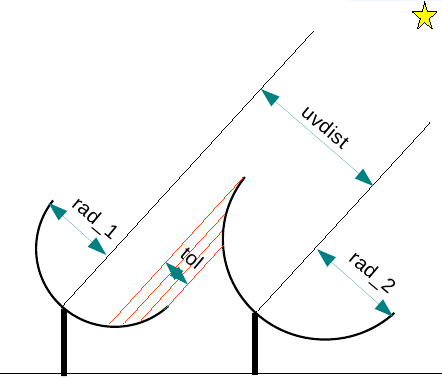
\includegraphics[scale=0.7]{shadow.diagram.png}
\caption{This figure shows the geometry used to compute shadowed antennas.}
\end{figure}



Note : The use of the phase-reference center as the pointing-direction for all antennas, is accurate in most 
cases, but will be approximate during on-the-fly mosaicing. However, since it is unlikely that an 
on-the-fly mosaic will be done with only one phase-reference center on a large-enough field-of-view
for shadow-flag differences to become significant.  


Note : Antennas that are not part of the MS ANTENNA subtable can be included in the calculation of
shadow flags by specifying a list of positions and diameters in an external file.   Note however that
the calculations will not account for the fact that antennas not part of
the observation, but still physically present on the ground, may not be pointing in the same direction as all the others
(as is assumed in the calculations).  If desired, the antenna diameters in the external file could
be adjusted accordingly.

Example : 
\begin{verbatim}
name=VLA1
diameter=25.0
Position=[-1601144.96146, -5041998.01971, 3554864.76811]

name=VLA2
diameter=25.0
position=[-1601105.76646, -5042022.39178, 3554847.24515]
\end{verbatim}

A helper-function has been provided to construct this list from an MS (possibly a different dataset)
that contains the required information in its ANTENNA subtable.

\begin{verbatim}
import flaghelper;
antlist =  flaghelper.extractAntennaInfo (
            msname='shadowtest.ms',
            antnamelist=['VLA1','VLA2','VLA9','VLA10'] );
flaghelper.writeAntennaList('antlist.txt',antlist);
\end{verbatim}


Figure \ref{ShadowExample} shows the flagging results from a simulated observation that spans a large
elevation range. Antennas near the center of the array are shadowed more than the others (left plot). 
If some antennas are split-out of the dataset, the ANTENNA subtable will have fewer antennas, and the shadow
flags will change (middle plot).  However, by specifying the positions and diameters of the missing antennas
via the external file, the correct shadow flags are recovered (right plot). 

\begin{figure}
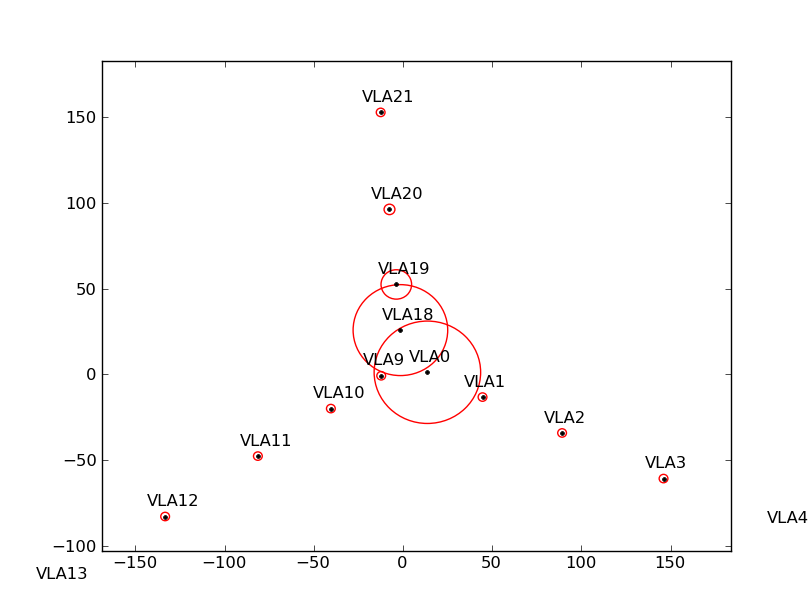
\includegraphics[scale=0.5]{plot.allants.shadow.png}
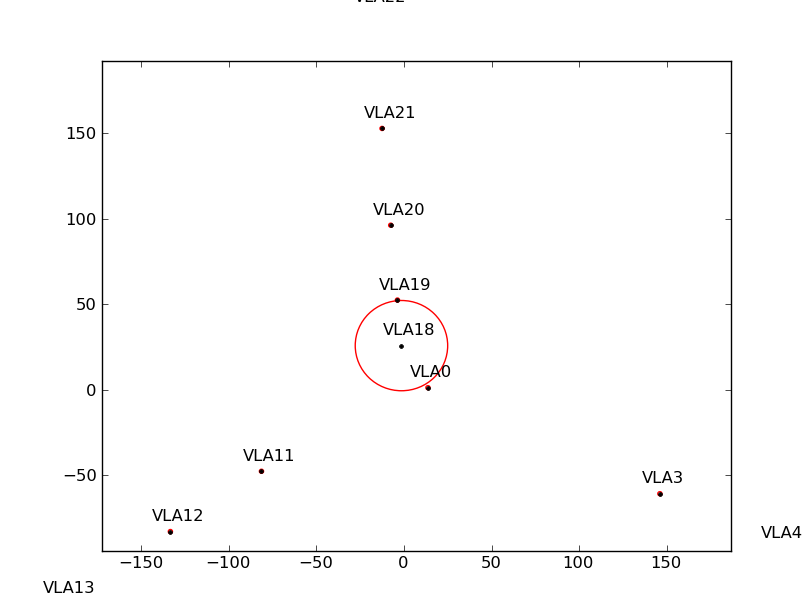
\includegraphics[scale=0.5]{plot.someants.shadow.png}
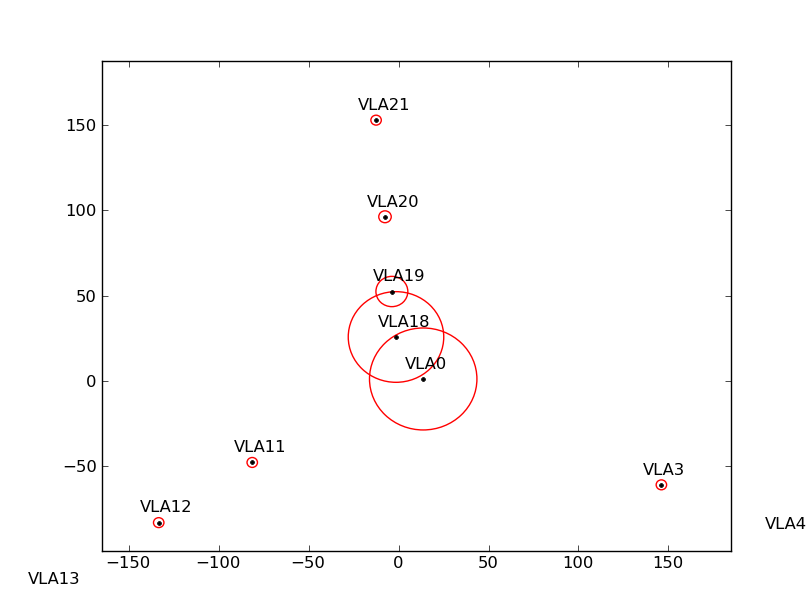
\includegraphics[scale=0.5]{plot.someants.withlist.shadow.png}
\caption{This figure shows  fractions of data flagged per antenna, for
three different use-cases. The size of the circle is proportional to the fraction of data flagged.
(LEFT) : Shadow-Flags with all antennas present in the MS,   (MIDDLE) : Shadow-Flags with four antennas (and their baselines) deleted from the MS,    (RIGHT) : Shadow-Flags from the MS with the missing antennas, but with the positions and diameters of the missing antennas specified via an external text file. The flags produced are the same as when all antennas are present in the MS.}
\label{Fig:ShadowExample}
\end{figure}


\subsubsection{TFCrop}

TFCrop is an autoflag algorithm that detects outliers on the 2D time-frequency plane, and 
 can operate on un-calibrated data (non bandpass-corrected).

The original implementation of this algorithm is described in 
\htmladdnormallink{NCRA Technical Report 202}{http://ncralib1.ncra.tifr.res.in:8080/jspui/handle/2301/127} (Oct 2003)


The algorithm iterates through the data in chunks of time.
For each chunk,  the result of user-specified visibility-expressions 
are organized as 2D time-frequency planes, one for each baseline 
and correlation-expression result, and the following steps are performed.

\begin{enumerate}
\item Calculate a bandshape template : 
Average the data across time, to construct an average bandpass.
     Construct an estimate of a clean bandpass (without RFI) via a
     robust piece-wise polynomial fit to the average bandpass shape.

       Note : A robust fit is computed in upto 5 iterations. 
It begins with a straight line fit across the full range, and gradually increases to 
     'maxnpieces' number of pieces with third-order polynomials in each piece. 
At each iteration, the stddev
                                between the data and the fit is computed, values beyond N-stddev are flagged,
                                and the fit and stddev are re-calculated with the remaining points.
                                This stddev calculation is adaptive, and converges to a value that reflects 
                                only the data and no RFI.  
At each iteration,  the same relative threshold is applied to detect flags, and this results in
a varying set of flagging thresholds,  that allows deep flagging only when the fit represents the true data best.
 Iterations stop when the stddev changes 
     by less than 10\%, or when 5 iterations are completed.

     The resulting clean bandpass is a fit across the base of RFI spikes.

\item  Divide out this clean bandpass function from all timesteps in the current chunk.  
Now, any data points that deviate from a mean of 1 can be considered RFI.  This step 
helps to separate narrow-band RFI spikes from a smooth but varying bandpass, in
situations where a simple range-based clipping will flag good sections of the bandpass.

\item Perform iterative flagging (robust flagging) of points deviating from a value of 1.  

  Flagging is done in upto 5 iterations. 
   In each iteration, for every timestep, calculate the stddev of the bandpass-flattened data, flag all points further than N times stddev from the fit, and recalculate the stddev.
 At each iteration,  the same relative threshold is applied to detect flags.
     Optionally, use sliding-window based statistics to calculate additional flags.

\item Repeat steps 1 and 3, but in the other direction (i.e. average the data across frequency,
     calculate a piece-wise polynomial fit to the average time-series, and find flags
     based on deviations w.r.to this fit.)

\end{enumerate}

The default parameters of the tfcrop implementation are optimized for strong narrow-band RFI.
With broad-band RFI, the piece-wise polynomial can sometimes model it as part of the
band-shape, and therefore not detect it as RFI.  In this case, reducing the maximum number 
of pieces in the polynomial can help.     This algorithm usually has trouble with
noisy RFI that is also extended in time of frequency, and additional statistics-based
flagging is recommended (via the 'usewindowstats' parameter).    It is often required to
set up parameters separately for each spectral-window.

If frequency ranges of known astronomical spectral lines are known $a-priori$, they can
be protected from automatic flagging by de-selecting those frequency-ranges via the 
'spw' data-selection parameter. 

Below are some examples that demonstrate what the algorithm does with different types
of RFI.

\begin{figure}
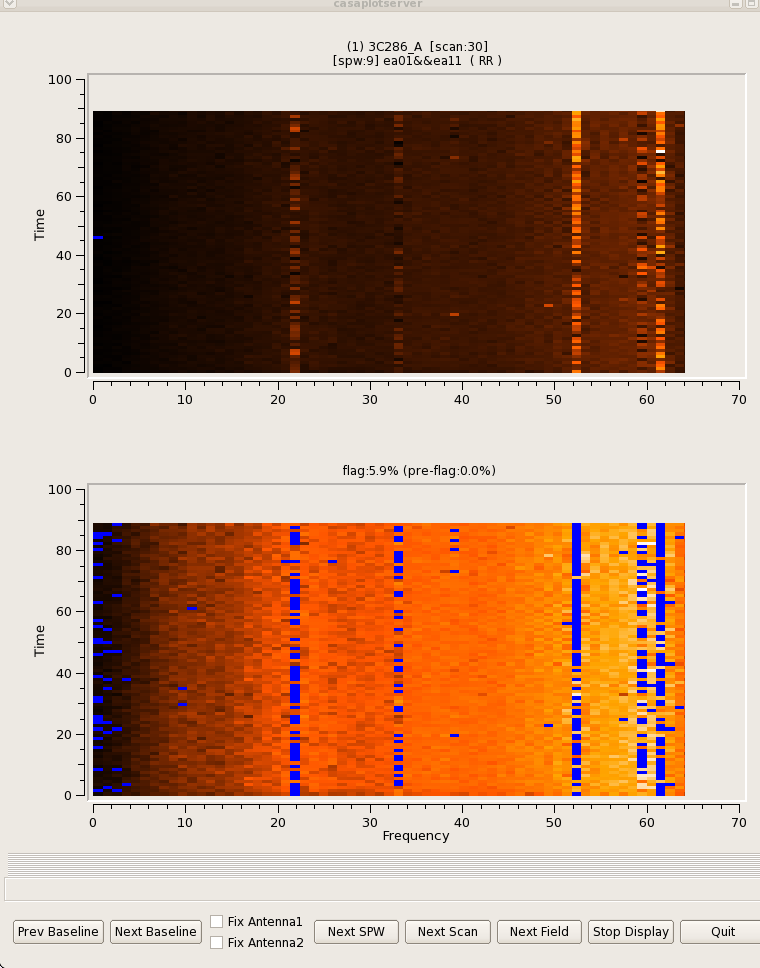
\includegraphics[scale=0.4]{flag.protect.specline.1.png}
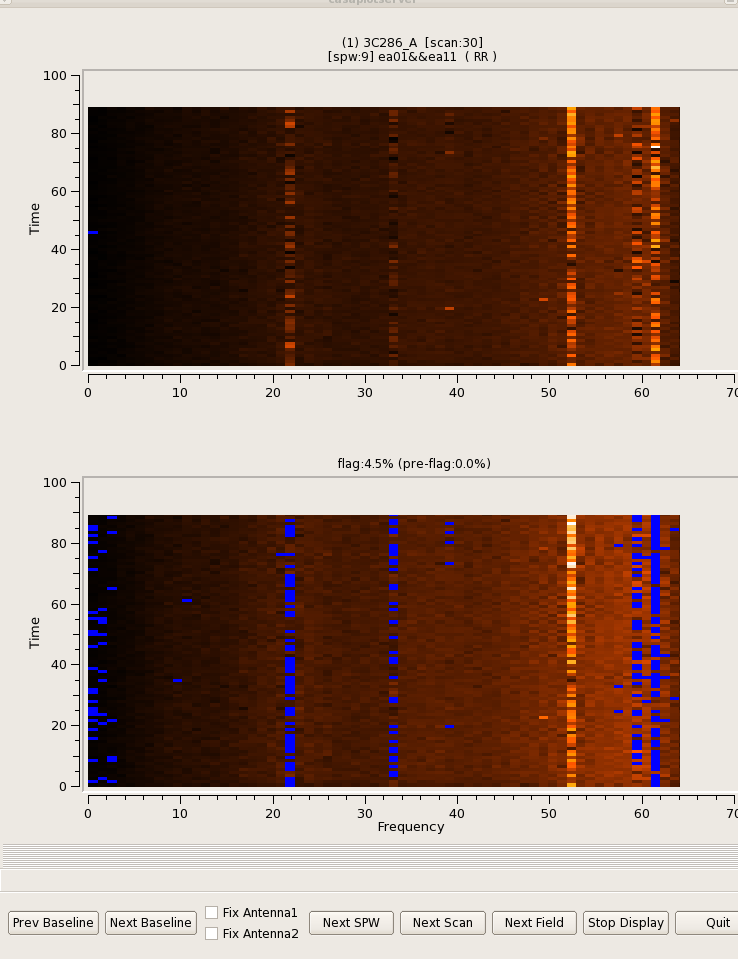
\includegraphics[scale=0.4]{flag.protect.specline.2.png}
\caption{LEFT : This screenshot represents a run where 'tfcrop' was run on a spw='9' with mainly narrow-band RFI.  RIGHT : An example of protecting a spectral line (in this case, demonstrated on an RFI spike) by setting the spw-selection to spw='0:0~45;53~63'.   In both figures, the top row indicates the data before flagging, and the bottom row after flagging.}
\end{figure}

{\red
FIG2 : Broad-band RFI
}


\subsubsection{RFlag}

RFlag is an autoflag algorithm based on a sliding window statistical filter (E.Greisen, AIPS, 2011).

The RFlag algorithm was originally developed by Eric Greisen in AIPS (31DEC11). \\
AIPS documentation : Subsection E.5 of the AIPS cookbook (\htmladdnormallink{Appendix E : Special Considerations for EVLA data calibration and imaging in AIPS}{http://www.aips.nrao.edu/cook.html#CEE})

In RFlag, the data is iterated-through in chunks
of time, statistics are accumulated across time-chunks, thresholds are calculated
at the end, and applied during a second pass through the dataset. 

The CASA implementation also optionally allows a single-pass operation where statistics
and thresholds are computed and also used for flagging, within each time-chunk
(defined by 'ntime' and 'combinescans'). 

For each chunk, calculate local
                         statistics, and apply flags based on user supplied (or auto-calculated) thresholds.

\begin{enumerate}
\item Time analysis (for each channel)
\begin{enumerate}
\item Calculate local rms of real and imag visibilities, within a sliding time window
\item Calculate the median rms across time windows, deviations of local rms from
                              this median, and the median deviation 
\item Flag if local rms is larger than timedevscale x (medianRMS + medianDev)
\end{enumerate}
\item Spectral analysis (for each time)
\begin{enumerate}

\item Calculate avg of real and imag visibilities and their rms across channels
\item Calculate the deviation of each channel from this avg, and the median-deviation
\item Flag if deviation is larger than freqdevscale x medianDev
\end{enumerate}

\end{enumerate}

{\red Add info about how to use 'writeflags' + 'display' + output thresholds, etc...}

Reports and plots are generated from rflag (when writeflags=False), to display
the mean deviations for each channel, as well as the mean variance of 
local statistics from this median deviation (local statistics are computed in a 
sliding-window). 


Below are some examples. 

\begin{enumerate}

\item Calculate thresholds automatically per scan, and use them to find flags.
                             Specify scale-factor for time-analysis thresholds, use default for frequency.

\begin{verbatim}
   tflagdata('my.ms', mode='rflag',spw='9',timedevscale=4.0,writeflags=True)
\end{verbatim}
 
\item  Supply noise-estimates to be used with default scale-factors. 
  
\begin{verbatim}
   tflagdata(vis='my.ms', mode='rflag', spw='9', timedev=0.1, freqdev=0.5, writeflags=True);
\end{verbatim}

\item Two-passes. This replicates the usage pattern in AIPS.

                             -- The first pass saves commands in an output text files, with auto-calculated thresholds.
                                Thresholds are returned from rflag only when writeflags=False (calc-only mode). 
                                The user can edit this file before doing the second pass, but the python-dictionary 
                                 structure must be preserved.

                             -- The second pass applies these commands (writeflags=True).

\begin{verbatim}
  tflagdata(vis='my.ms', mode='rflag', spw='9,10',                                               timedev='tdevfile.txt', freqdev='fdevfile.txt', writeflags=False);
  tflagdata(vis='my.ms', mode='rflag', spw='9,10', 
            timedev='tdevfile.txt', freqdev='fdevfile.txt', writeflags=True);
\end{verbatim}
            
\end{enumerate} 


\begin{figure}
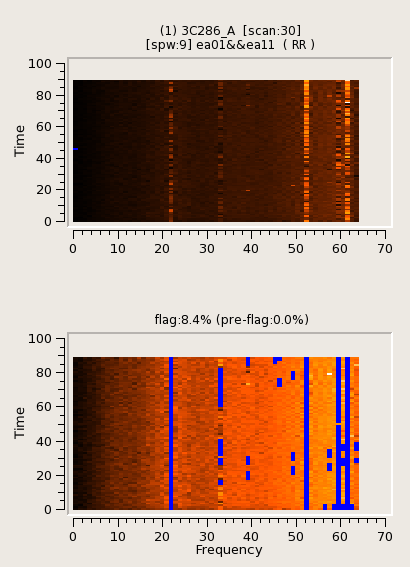
\includegraphics[scale=0.8]{rflag.before.after.png}
\caption{Example of rflag on narrow-band RFI}
\end{figure}

{\red Add figures of the new report plots.}

\subsubsection{Extend}

Flags can be extended along various axes (within one spw, field, and time-chunk). 
Autoflag algorithms on their own often leave out pieces of RFI-affected data, in-between flagged
points, and flag extensions are often useful.  Data points can be flagged if more than half of 
the surrounding points are already flagged.  If a timerange or frequency-range is more than 
(for example) 50\% flagged, the entire range can be flagged.  Flags can be extended across
correlations, in cases where the RFI-signal-to-noise ratio is higher in some correlations where
it is easier to detect than in other correlations. 

\begin{figure}
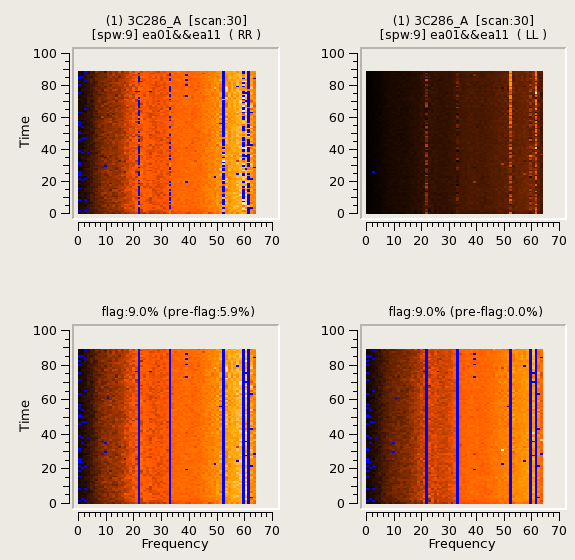
\includegraphics[scale=0.8]{flag.extension.png}
\caption{This screenshot represents a run where 'tfcrop' was run only on
'ABS\_RR' (top row) and followed by an extension along time and correlations
(bottom row). }
\end{figure}


%%%%%%%%%%%%%%%%%%%%%%%%%%%%%%%%%%%%%%%%%%%%%%%%%%%%
%%%%%%%%%%%%%%%%%%%%%%%%%%%%%%%%%%%%%%%%%%%%%%%%%%%%


\subsection{List of flag commands (tflagdata, flagcmd)}
\label{Sec:FlagCmdLists}
There are two flagging tasks in version 3.4 of CASA. The main task tflagdata is
a replacement for the old flagdata/flagdata2/testautoflag/flagautocorr. This
task can take parameters input from the interface as well as input from an
external text file. This is the so-called list mode. All the flagging commands
that apply to an MS can be combined into one single text file and read in for
processing. Only the summary mode is not allowed in list mode to avoid
confusion when several summaries are present in the list. The user can run
tflagdata separated to get the summary of the list. 

The other task, flagcmd is a replacement for the previous version of flagcmd. It
has a re-factored interface and it can do much more than the previous version.
All the flagging modes available in tflagdata are also allowed in flagcmd
(except again for the summary mode). Several input modes are available: table,
file, xml and cmd. Actions to perform on the input are: apply, unapply, list,
clear, plot and extract.

\subsubsection{Apply/ un-apply}
It is possible to truly unapply flag commands in flagcmd. In order to guarantee that only the data selected in 
the commands is unapplied, the framework will first unapply the selected rows
and then re-apply the overlapping data that got unapplied in the first pass. This is a true unapply action, but it will take longer to
process because it will re-apply all the remaining commands that have the
column APPLIED set to True inside the FLAG\_CMD sub-table of the MS.

\subsubsection{Using flag-commands in the flagcmd task}
Flag commands can be given as input to the flagcmd task in several ways. The
default is the 'table' which will have the flag commands inside the FLAG\_CMD
sub-table of the MS in a column called COMMAND.

The other input, as already detailed above is the 'file' mode, which will have
the flag commands in a text file.

The 'xml' input is meant to be used for the online flags from the Flag.xml file
in the MS. It also assumes that the Antenna.xml file is present.

The last input mode will input the flag commands from a list of Python strings.

For all the input modes, the action='list' can be used to list the flags
commands on the screen and optionally to save them to an external output file
when the parameter savepars is set to True.

When the action='apply' is used in the inpmode table, the flags will be applied
to the MS and the APPLIED column will be updated to True. On the other hand,
when action='unapply' the APPLIED column will be set to False for all selected
table rows.

\paragraph{Examples}

\begin{enumerate}
\item Input commands from the FLAG\_CMD sub-table. 

\begin{figure}
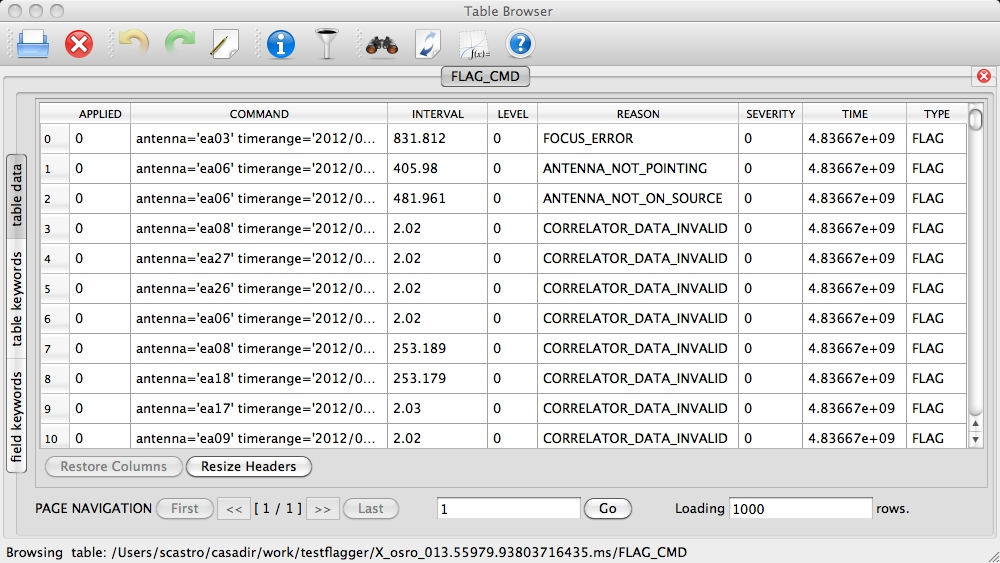
\includegraphics[scale=0.8]{flagcmd_screenshot.png}
\caption{Screenshot of the FLAG_CMD sub-table of a MS with flag commands for the
online flags. }
\end{figure}

\begin{verbatim}
# Apply only the flag commands that contain reason='CORRELATOR_DATA_INVALID'.
The default action for flagcmd is to apply the flag commands from a table input,
therefore it is not necessary to specify inpmode='table' and action='apply'.

 flagcmd(vis='uid.ms', reason='CORRELATOR_DATA_INVALID')
  
\end{verbatim}

\item Input commands from an ASCII file.
\begin{verbatim}
# Create an input text file with all the flag commands to apply to the MS.
> cat flags.txt
 mode='manual' autocorr=True
 mode='shadow'
 mode='clip' clipminmax=[0,2] clipzeros=True correlation='ABS_ALL'
 mode='tfcrop' spw='9' correlation='ABS_YY' ntime=51.0
 mode='extend' extendpols=True

# Pass the input to the task
  flagcmd(vis='uid.ms', inpmode='file', inpfile='flags.txt', action='apply')
 
\end{verbatim}

\item Input commands via a list of strings.
\begin{verbatim}
# Create a Python string called mycmd.
  flagcmd(vis='uid.ms', inpmode='cmd',
          command=["mode='manual' autocorr=True",
                   "mode='shadow'",
                   "mode='clip' clipminmax=[0,2] clipzeros=True correlation='ABS_ALL'", 
                   "mode='tfcrop' spw='9' correlation='ABS_YY' ntime=51.0",
                   "mode='extend' extendpols=True"], action='apply')
 
 
\end{verbatim}
\end{enumerate}

\subsubsection{Using flag-commands in the tflagdata task}

\paragraph{Examples}

\begin{enumerate}
\item Run tflagdata in list mode, using a flag-command file.

\begin{verbatim}
# Create an input text file with all the flag commands to apply to the MS.
> cat flags.txt
 mode='manual' autocorr=True
 scan='1~3' mode='manual'
 mode='clip' clipminmax=[0,2] clipzeros=True correlation='ABS_ALL'
 mode='tfcrop' spw='9' correlation='ABS_YY' ntime=51.0
 mode='extend' extendpols=True

# Pass the input to the task
  tflagdata(vis='uid.ms', mode='list', inpfile='flags.txt')
 
# Get a summary
  tflagdata(vis='uid.ms', mode='summary')

\end{verbatim}

\item Select by reason in list mode.

\begin{verbatim}
# Apply only the flag commands that contain reason='BAD_ANT'. Let's say the
input file contains the following flag commands.

> cat flags.txt
  antenna='DV06' reason='BAD_ANT'
  mode='clip' clipzeros=True reason='CLIPZEROS'
  mode='shadow' reason='SHADOW'
  antenna='DV01' timerange='2012/02/01:09:14:0~09:54:0' reason='BAD_ANT'
  antenna='DV10;DV23' timerange='2012/02/01:09:15:0~09:54:0' reason='BAD_ANT'
  
 # We want to apply the above flag commands in three different MSs, but in the
 first step we only want to flag the bad antennas, so we will select the cmds
 by the reason given in the file.
 
   tflagdata(vis='uid1.ms', inpmode='list', inpfile='flags.txt',
             reason='BAD_ANT')

   tflagdata(vis='uid2.ms', inpmode='list', inpfile='flags.txt',
             reason='BAD_ANT')

   tflagdata(vis='uid3.ms', inpmode='list', inpfile='flags.txt',
             reason='BAD_ANT')
      
\end{verbatim}

\item Saving the parameters as flag commands, to a file.

\begin{verbatim}
# Sometimes we want to flag using the interface but would like to save those
parameters to a file. It may also be useful to write along a reason for those
flags.

  tflagdata(vis='uid1.ms', mode='clip', clipzeros=True, savepars=True,
            outfile='myflagcmd.txt', cmdreason='CLIPZEROS')
  
# This will flag all the zeros in the MS and save the parameters to
'myflagcmd.txt' like below:

> cat myflagcmd.txt
mode='clip' correlation='ABS_ALL' clipoutside=True datacolumn='DATA'\
channelavg=False clipzeros=True reason='CLIPZEROS'

# NOTE: if the outfile is left empty (default case), the task will save the
parameters to the FLAG_CMD sub-table.

\end{verbatim}
\end{enumerate}


\paragraph{Using (and mis-using) the FLAG_CMD subtable}
The FLAG\_CMD sub-table is meant to store only meta-data selections such as
online flags. Using it to save other parameters (from modes such as clip, quack,
shadow, etc.) is possible but carries a risk that in future releases these
these parameters or their default values are renamed or changed.
Use it at your own risk! There will be no automatic way to rename any parameter that changes in the
future.

Keeping the state of the flags stored in the FLAG\_CMD sub-table is also not
guaranteed. The state can get out-of-sync very easily with the interchangeable
use of all flagging tasks such as tflagdata, flagcmd, and interactive
flagging using plotms. Note that plotms does not write to the FLAG\_CMD
sub-table.

%%%%%%%%%%%%%%%%%%%%%%%%%%%%%%%%%%%%%%%%%%%%%%%%%%%%
%%%%%%%%%%%%%%%%%%%%%%%%%%%%%%%%%%%%%%%%%%%%%%%%%%%%

\subsection{Summaries, displays, reports}

\subsubsection{Flag summaries}

Screenshot of runtime flag 
\begin{figure}
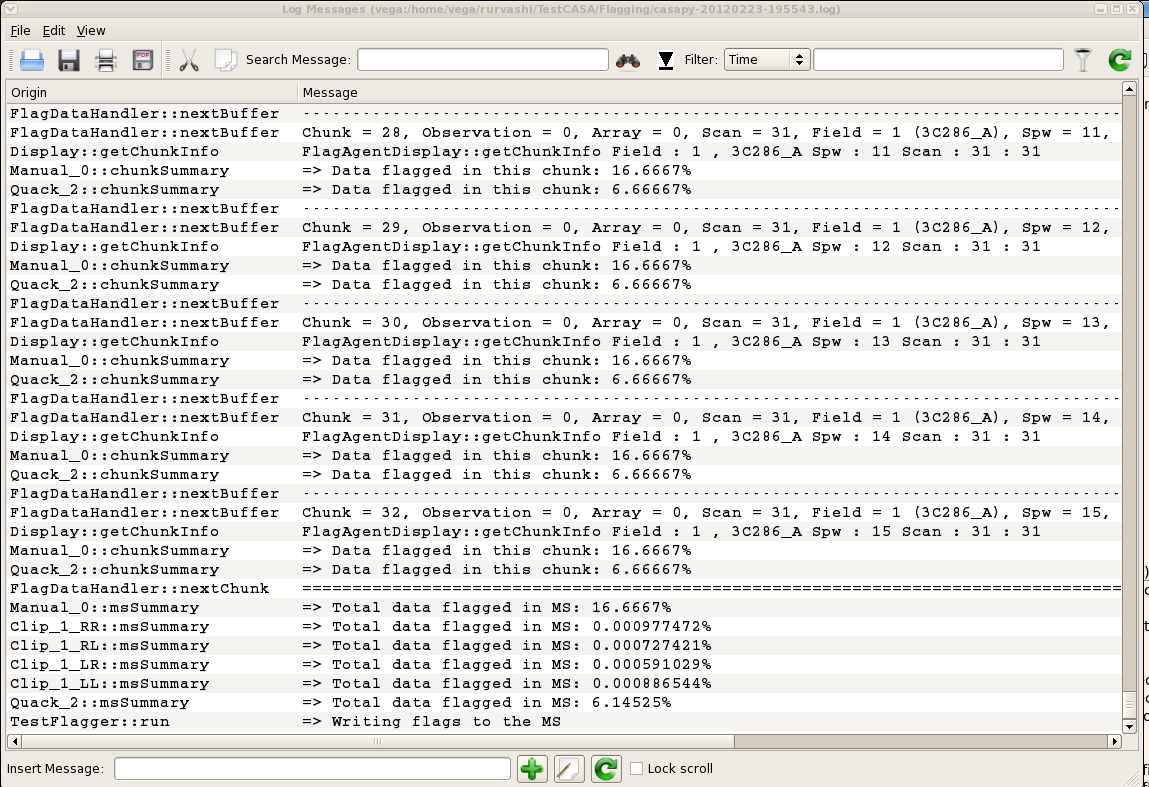
\includegraphics[scale=0.7]{flag.screenshot.logger.png}
\caption{Example of runtime logger summary of flag counts per agent}
\end{figure}

Flag count dictionaries : {\red verbatim output of part of one...}



\subsubsection{Flag Reports/Views}

Here are some examples of flag report displays on two datasets.
\begin{enumerate}
\item Percentage of data flagged vs frequency : To assess how much usable data is present in each spectral-window, for later processing, and imaging sensitivity-estimates.
\item Percentage of data flagged vs antenna-position : To assess whether the RFI is restricted to only some antennas and therefore may be local.
\item Percentage of data flagged vs baseline-length : To assess expected sensitivities for different spatial scales, since local RFI correlates better on shorter baselines than longer ones.
\end{enumerate}

\subsubsection{Data Display + action='calculate'}
In order to visualize some of the RFI present in the data, and to verify if flagging
commands are having the desired effect,  there is an option to 
visualize the data and flags at run-time, and navigate between baselines in the 
current chunk, as well as in the forward-direction across scans and spws.   

The intended usage of the display is to run the flagger on small subsets of the data (sub-selections)
with action='calculate', and display='data', and inspect the flagging results. 
An option to quit at any stage allows the user to change input parameters and try again until the
desired flagging results are obtained.  Then, the display can be turned off,
action set to 'apply', and the program run again on a larger section of the
data.


\subsection{Flagging Calibration-Tables}
{\green  Anything specific to calibration tables.   } 


\section{Frequently Asked Questions}

\subsection{Obtaining summaries per reason}
Attach the tool script that does this.

\subsection{FLAGCMD sub-table vs flag-command text files}
See section \ref{Sec:FlagCmdLists}


\subsection{Will batch modes make the flagging faster ?}

Batch operations will help only if data and flag I/O is shared between the flag commands.  
If commands touch different data-selections, running them together will not help.

\begin{enumerate}
\item The following sequence of operations will benefit from being run together, 
because they all access spw 9, clip and rflag read visibilities, and rflag and extend read flags:

mode='manual'  spw='9:0~3;61~63' \\
mode='clip'  clipminmix=[0.0, 1e+5] \\
mode='rflag'   spw='9' \\
mode='extend'  growtime=80.0   extendpols=True 

\item This is an example that will not benefit from the list mode : 

mode='manual'  spw='9:0~3;61~63' \\
mode='clip'  spw = '5'  clipminmix=[0.0, 1e+5] 

\end{enumerate}




\subsection{Comparison of RFI with 1s vs 10s integrations}
In order to reduce dataset sizes, data can be averaged during the observation. However, with integration-times of anything larger than few seconds, there is the risk of smearing out the RFI and losing a larger fraction of the data to RFI.   

The following is the result of a few autoflag tests on an L-Band D-config 7-hour dataset (G55.7+3.4), for which we have a version with 1sec integrations,a 10s averaged version (with and without pre-applying online flags).

%, and a set of flags created by hand on one of the 10sec averaged versions. 

Figures \ref{Fig:compare_1} and \ref{Fig:compare_2} show the percentage of data flagged per frequency-channel for the 1sec and 10sec datasets respectively, showing a few\% less data flagged in the 10sec dataset.  Figures \ref{Fig:compare_3} and \ref{Fig:compare_4} show the percentage flagged per antenna and scan (each scan is 1.5 minutes long), and show a difference of about 1\% in the amount of data flagged by 'rflag', indicating that there is no practical loss of data due to smearing out of the RFI during the 1sec-to-10sec averaging. 
Figure  \ref{Fig:compare_5} is the result of applying online flags on the 1-sec data before averaging to 10-sec and running rflag. Comparing with the previous plots, this saves about 1\% to 2\% of the flagged data. 

Figure  \ref{Fig:compare_6} shows plots of the un-calibrated data for the first two cases (1sec and 10sec), to demonstrate that 'rflag' has identified RFI correctly in both cases. Note that the 1-sec data were averaged for the purpose of plotting (after flagging).

These quick tests and summaries show that from the point of view of RFI-identification and flagging, there is no advantage of recording data at a 1-sec for D-Config and L-Band. In general, it should suffice if averaging rules follow time-smearing limits at any given configuration.

\begin{figure}
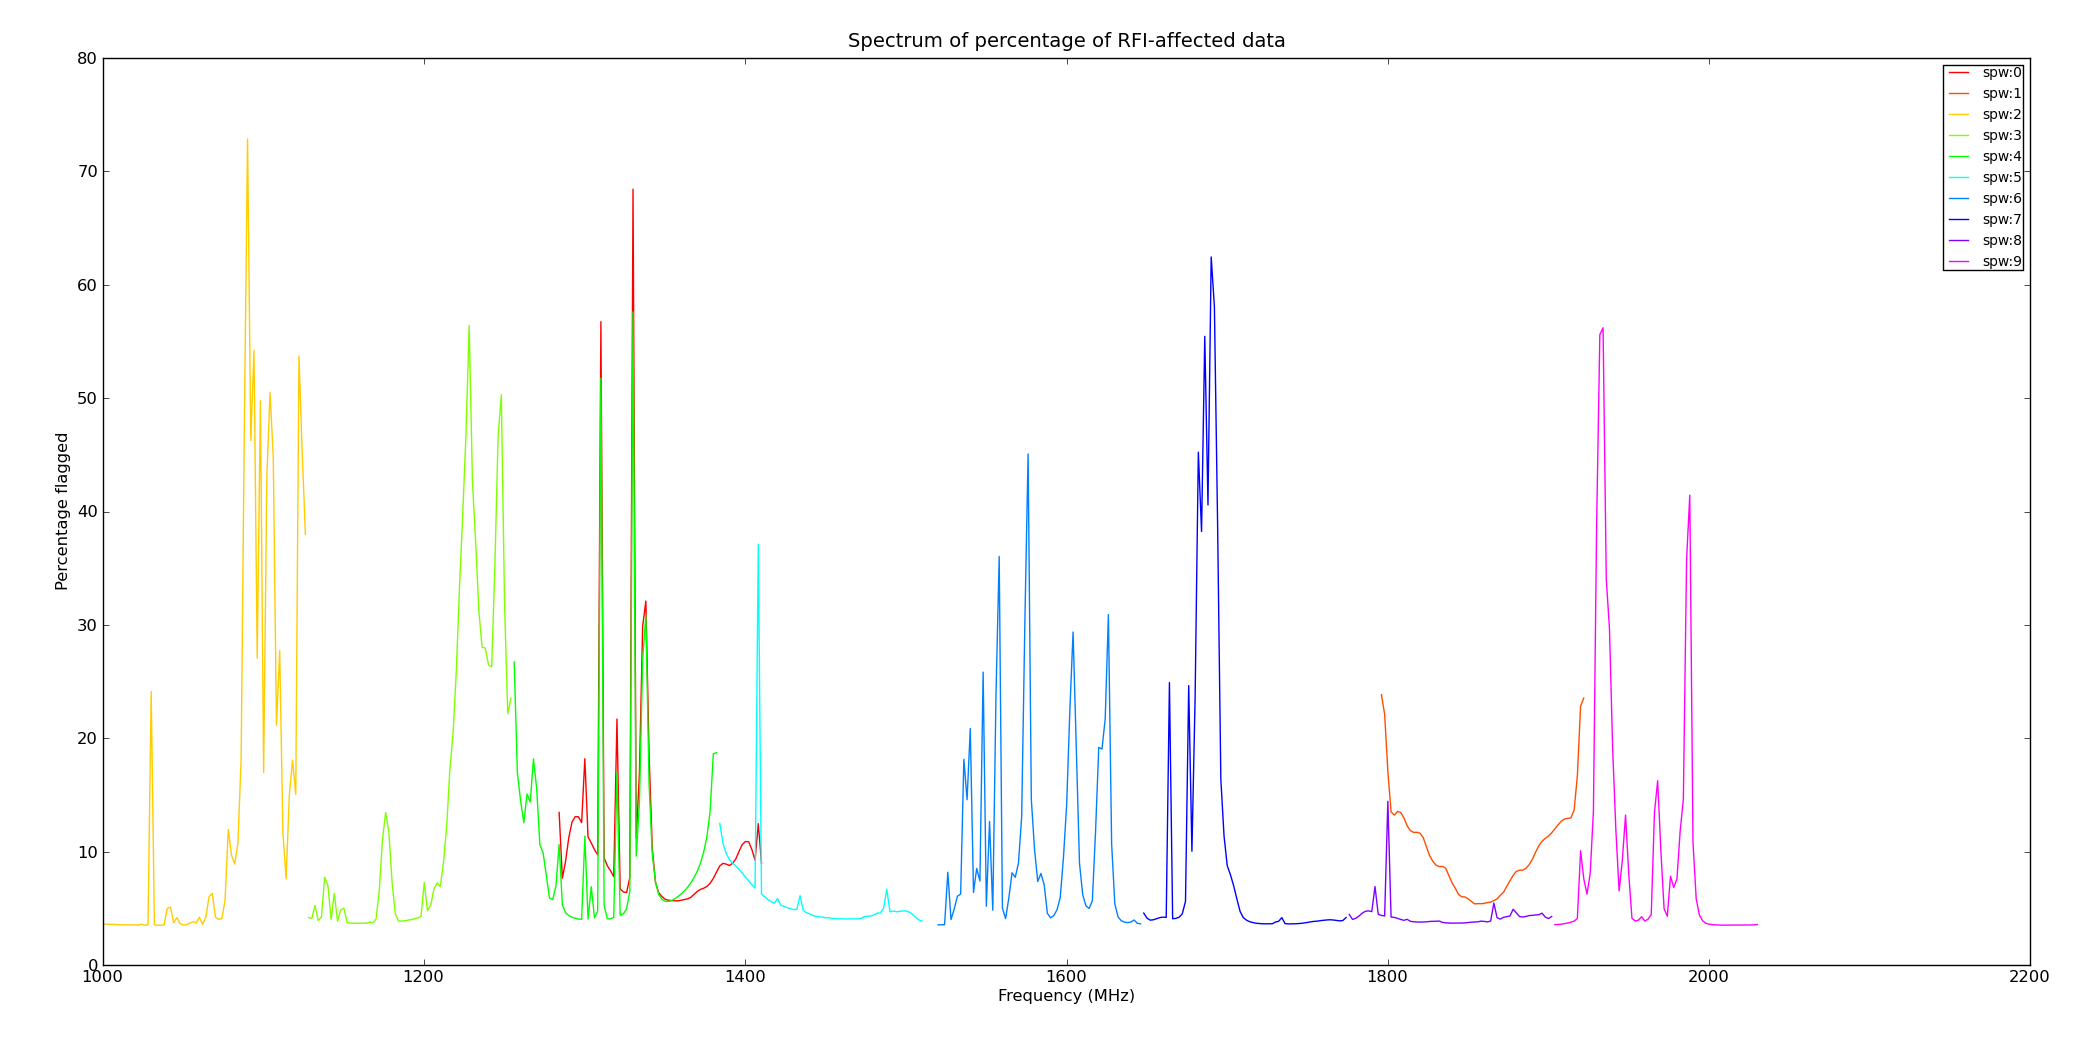
\includegraphics[scale=0.5]{plot.anttime.G55.1s.freqplot.png}
\caption{Plots of the percentage flagged per channel :  Dataset with 1sec timesteps.}
\label{Fig:compare_1}
\end{figure}

\begin{figure}
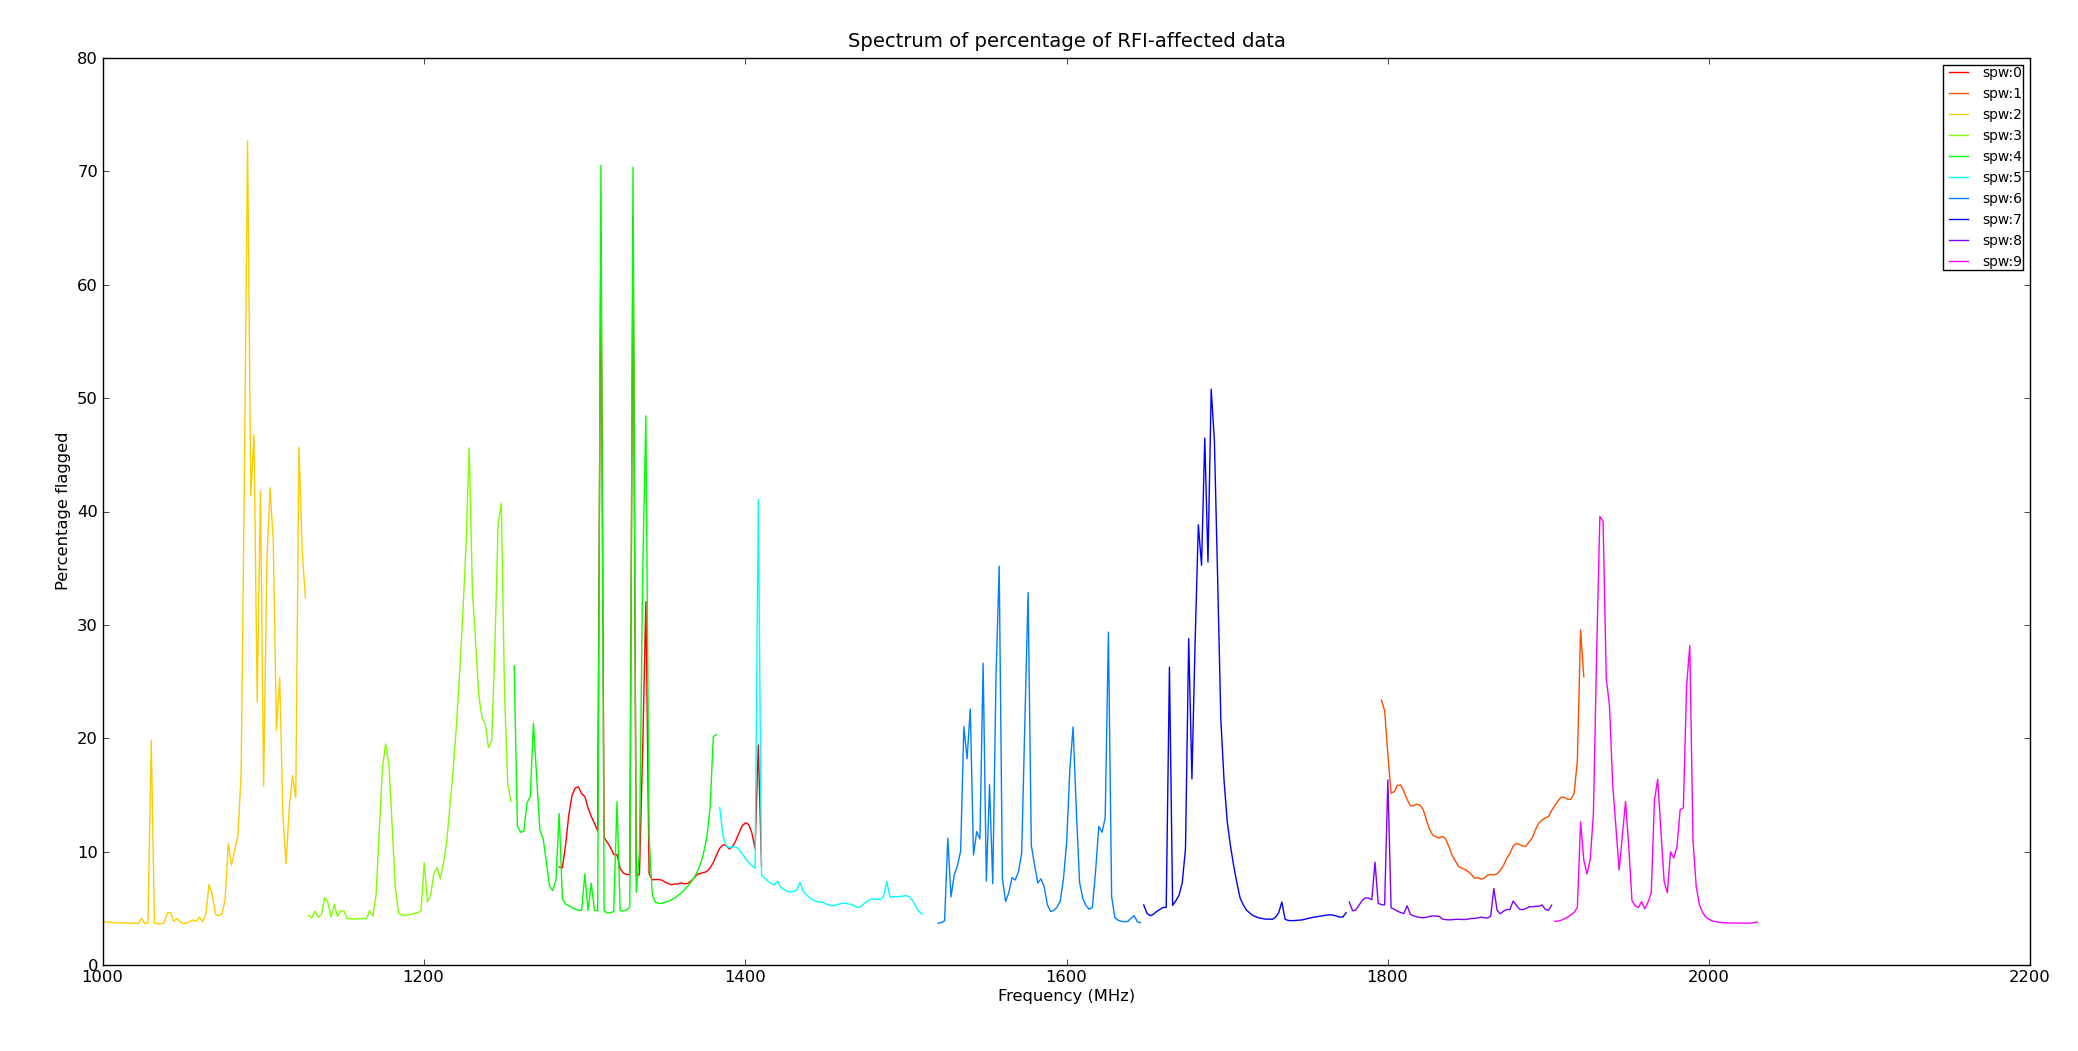
\includegraphics[scale=0.5]{plot.anttime.G55.averaged.10s.freqplot.png}
\caption{Plots of the percentage flagged per channel : Dataset with 10sec timesteps.}
\label{Fig:compare_2}
\end{figure}

\begin{figure}
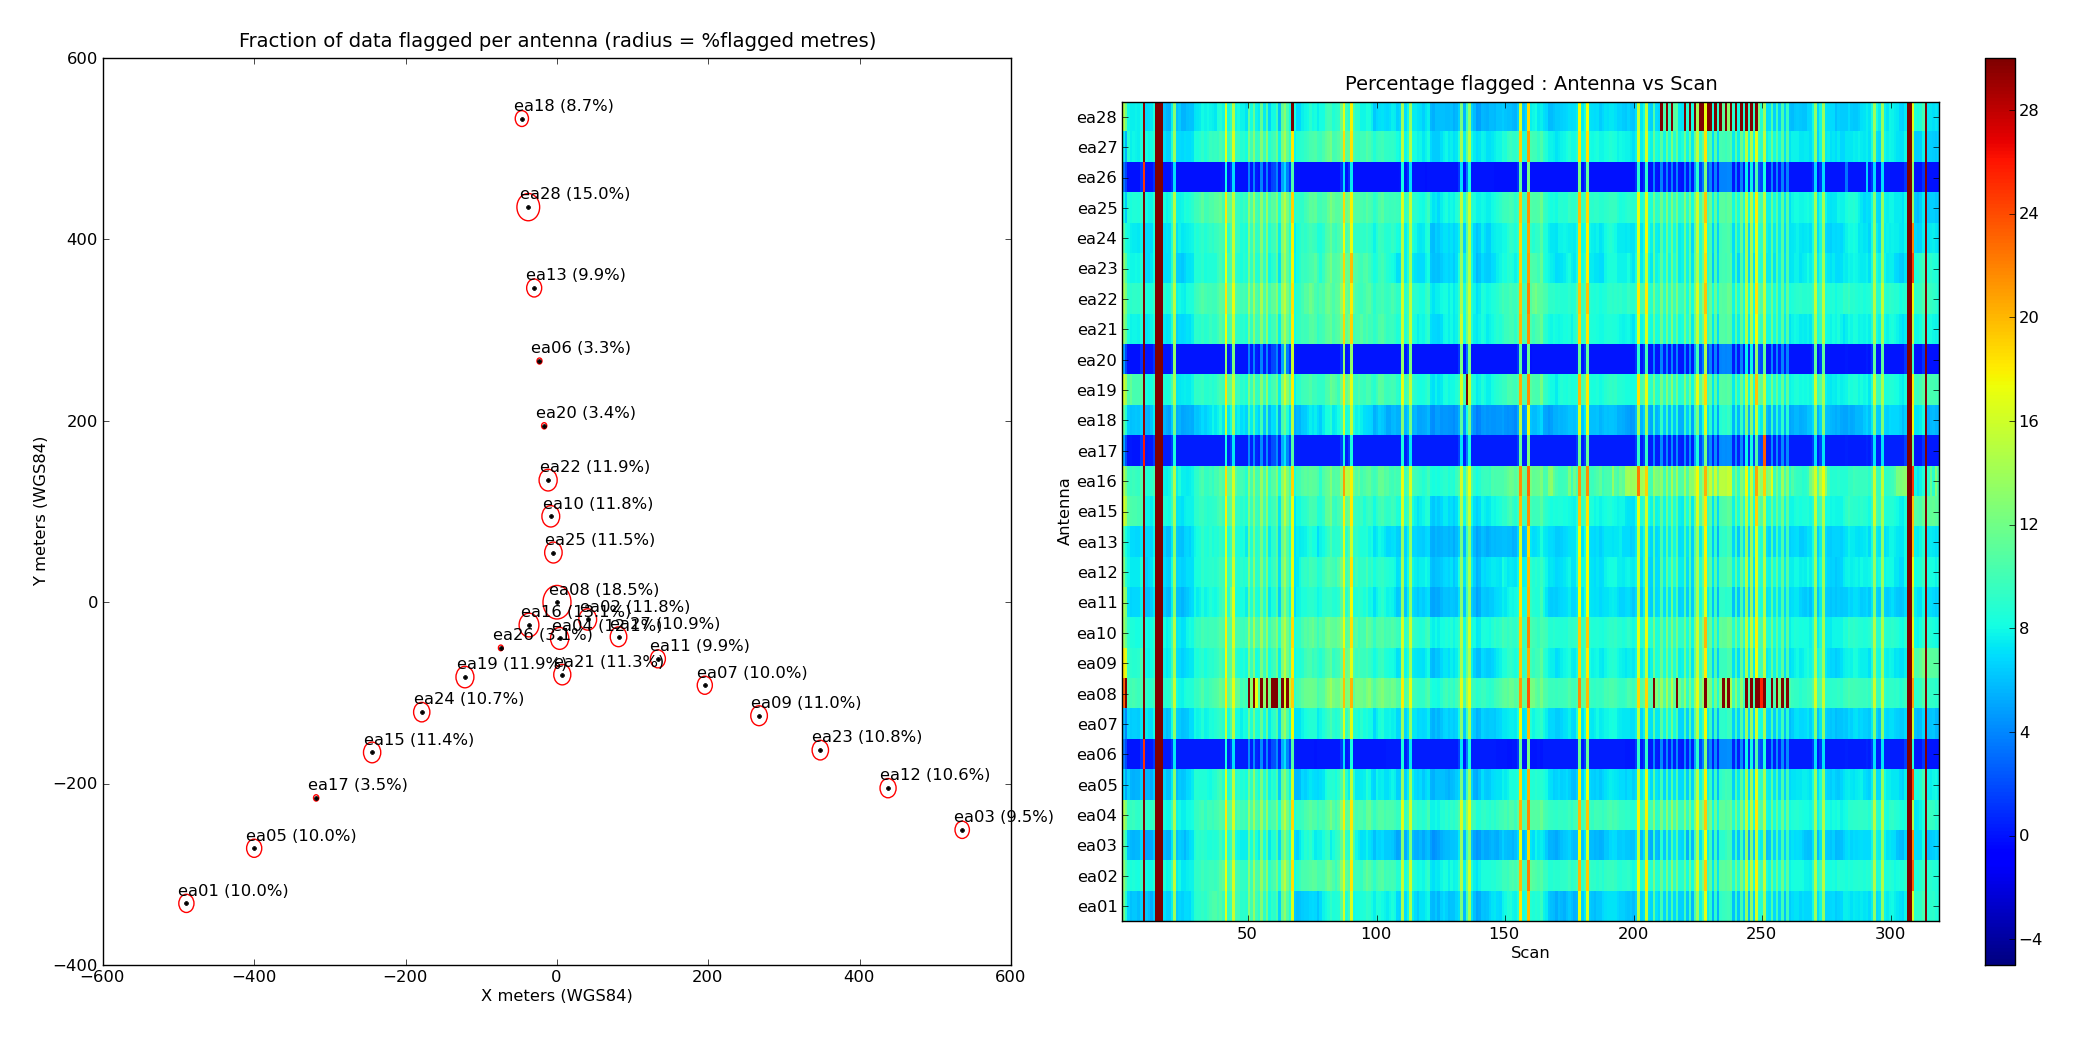
\includegraphics[scale=0.5]{plot.anttime.G55.1s.scanplot.png}
\caption{Dataset with 1sec timesteps : Plots of the percentage flagged per antenna and scan. Each scan is about 1.5 minutes long. Flagging includes online flags followed by rflag running per scan. The left panel shows the percentage flagged per antenna, over all scans.}
\label{Fig:compare_3}
\end{figure}

\begin{figure}
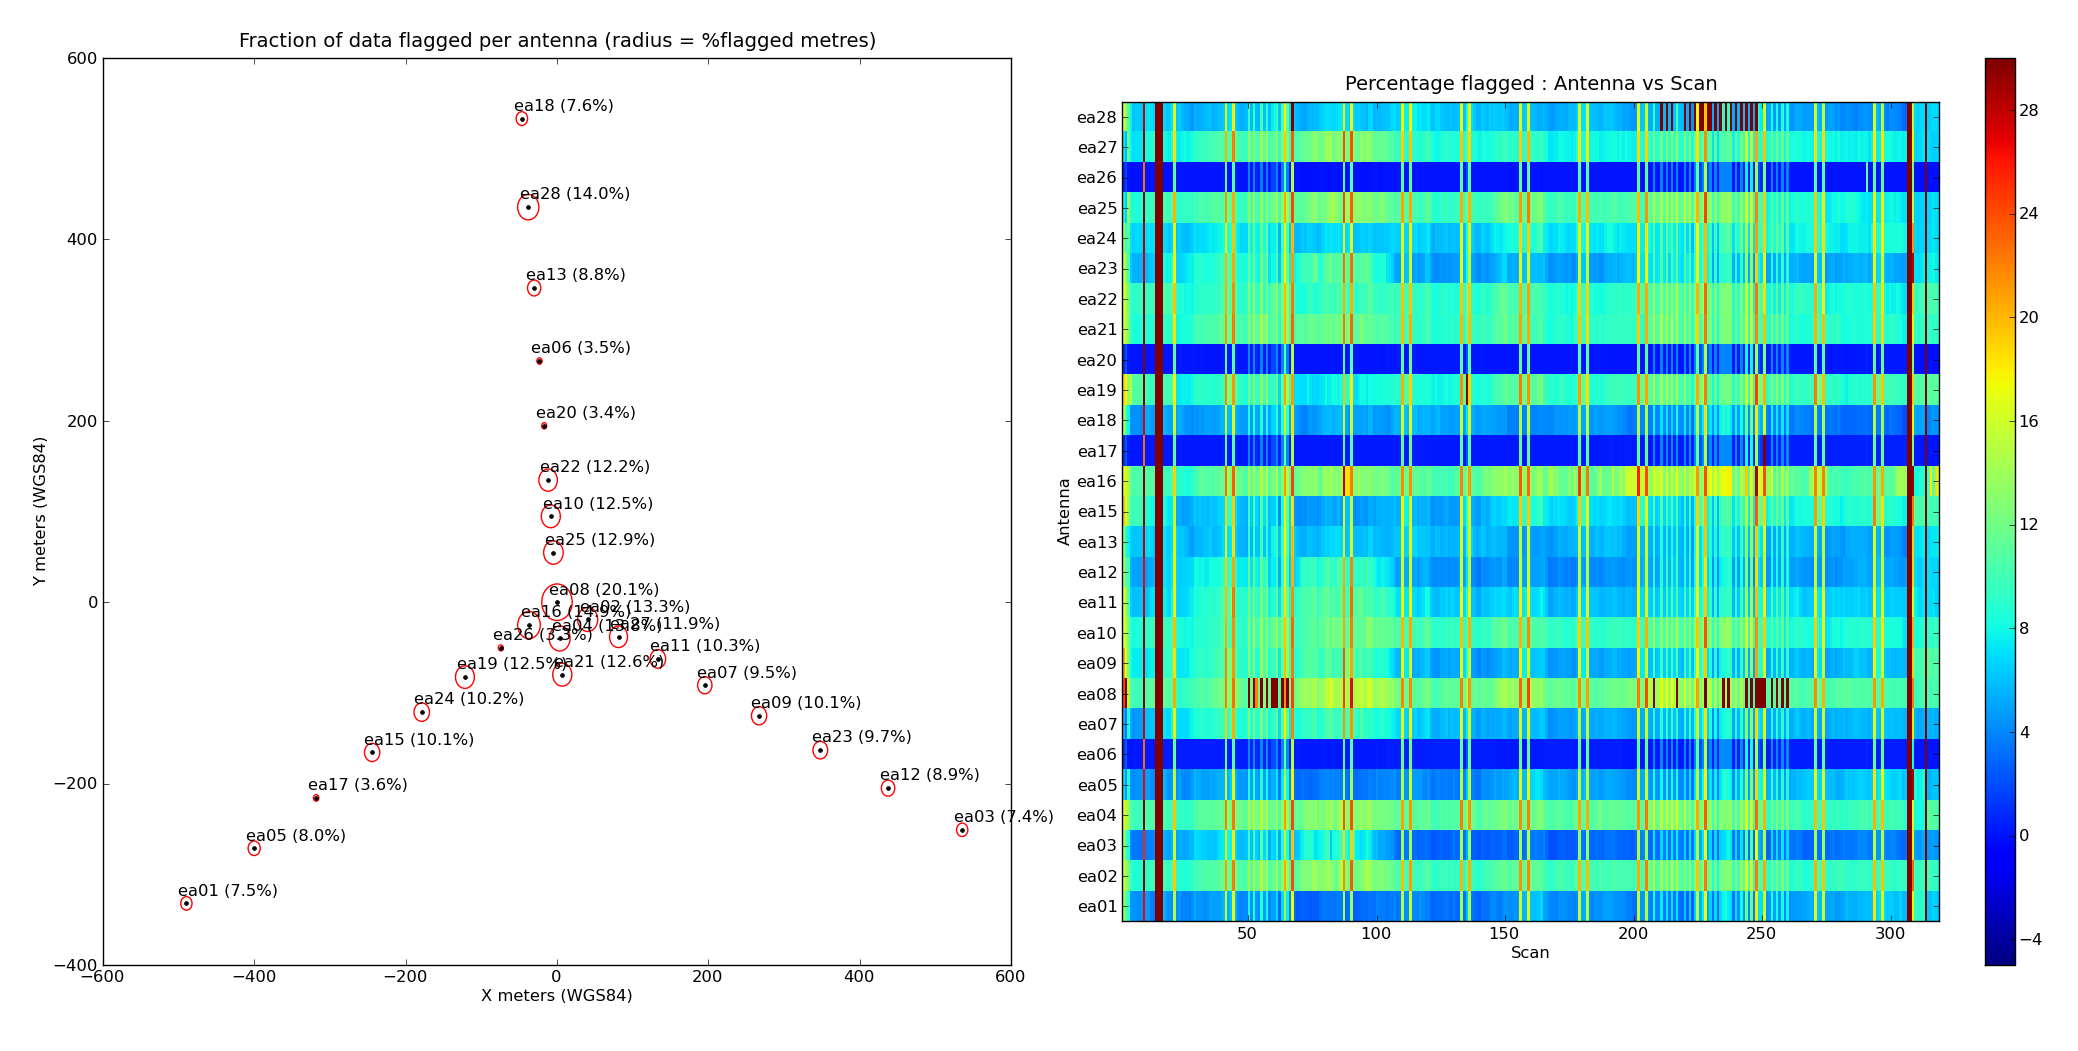
\includegraphics[scale=0.5]{plot.anttime.G55.averaged.10s.scanplot.png}
\caption{Dataset with 10sec timesteps : Plots of the percentage flagged per antenna and scan. Each scan is about 1.5 minutes long. Flagging includes online flags followed by rflag running per scan. The data was completely unflagged before averaging to 10sec, to simulate averaging within the correlator.}
\label{Fig:compare_4}
\end{figure}

\begin{figure}
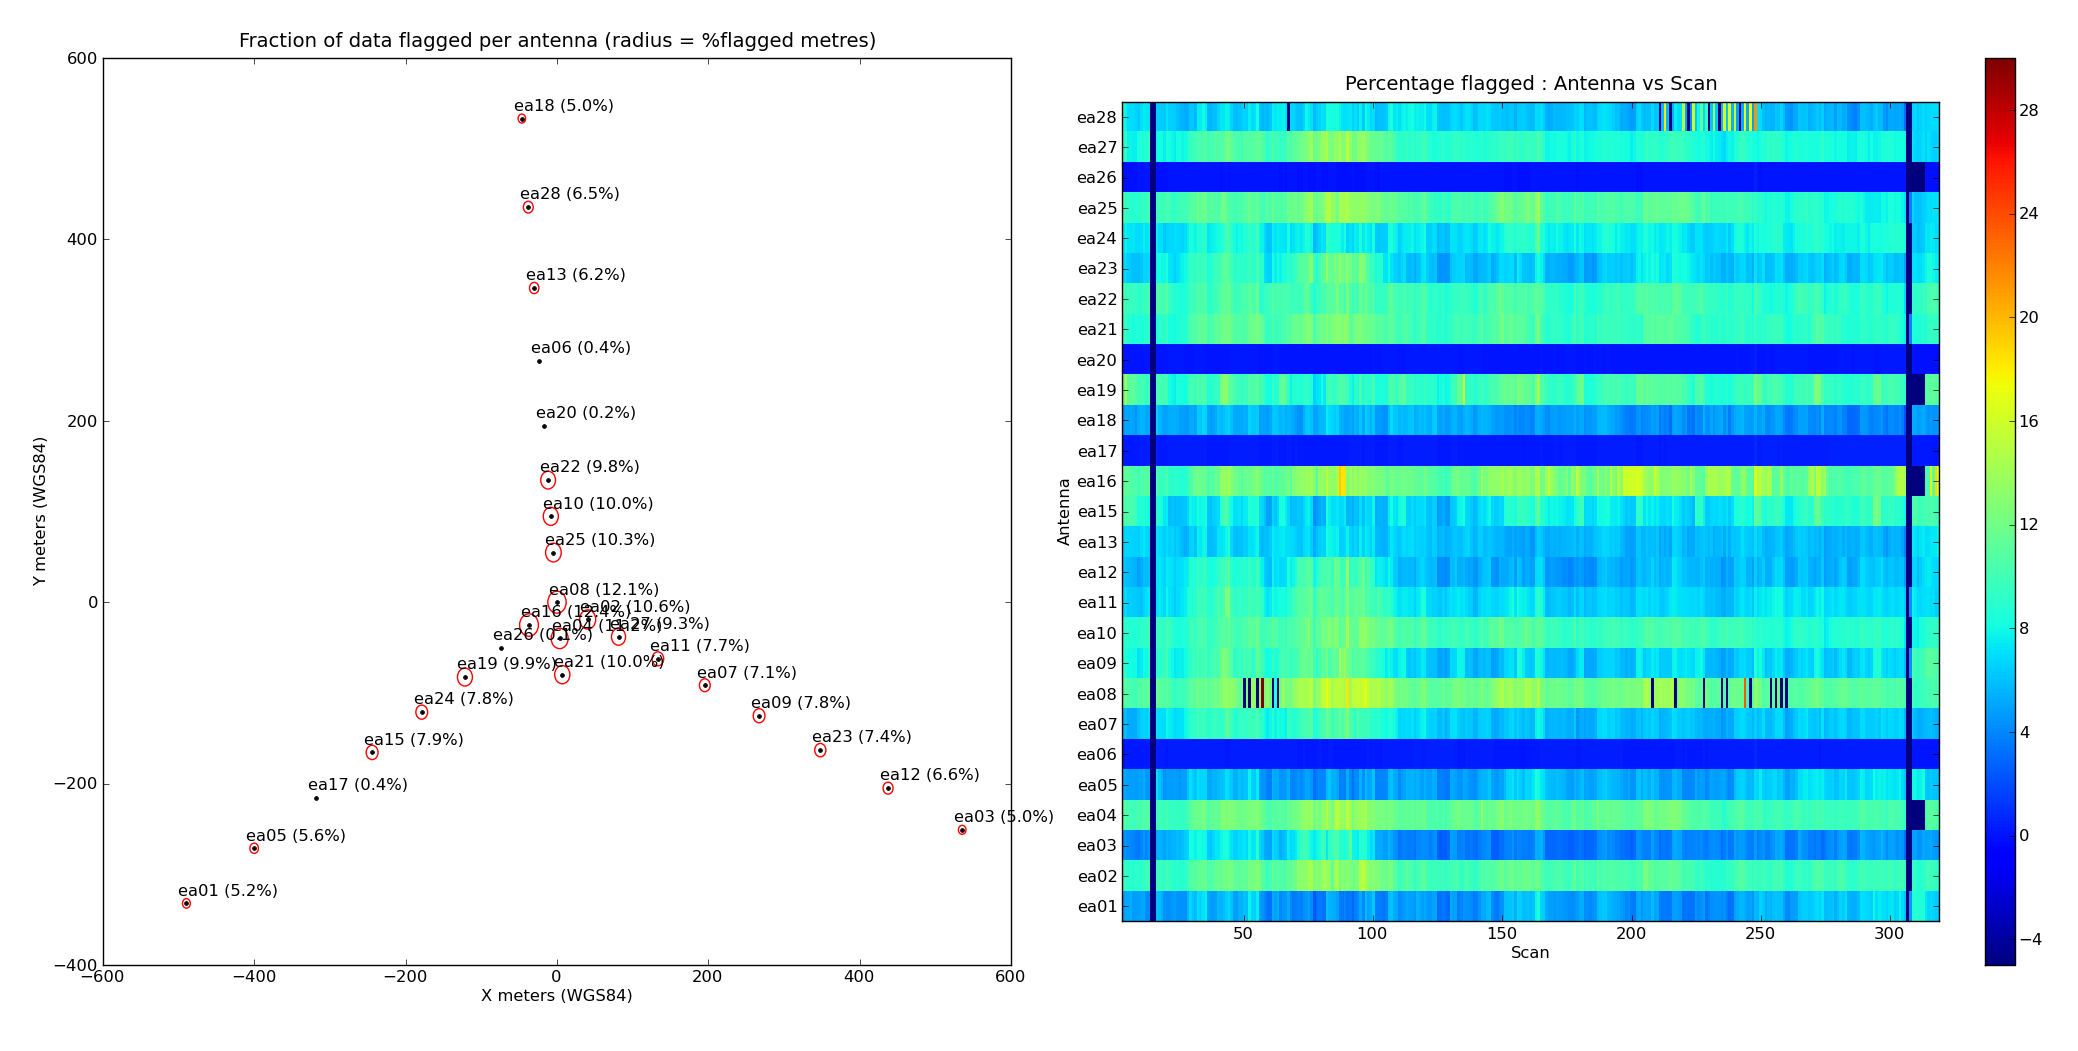
\includegraphics[scale=0.5]{plot.anttime.G55.10s.scanplot.png}
\caption{Dataset with 10sec timesteps, with online flags applied before averaging from 1sec to 10sec.  Plots of the percentage flagged per antenna and scan. Each scan is about 1.5 minutes long. Comparing with the previous two plots, again, there is very little gain (about 2\% of data) of applying online flags before averaging to 10sec. }
\label{Fig:compare_5}
\end{figure}


\begin{figure}
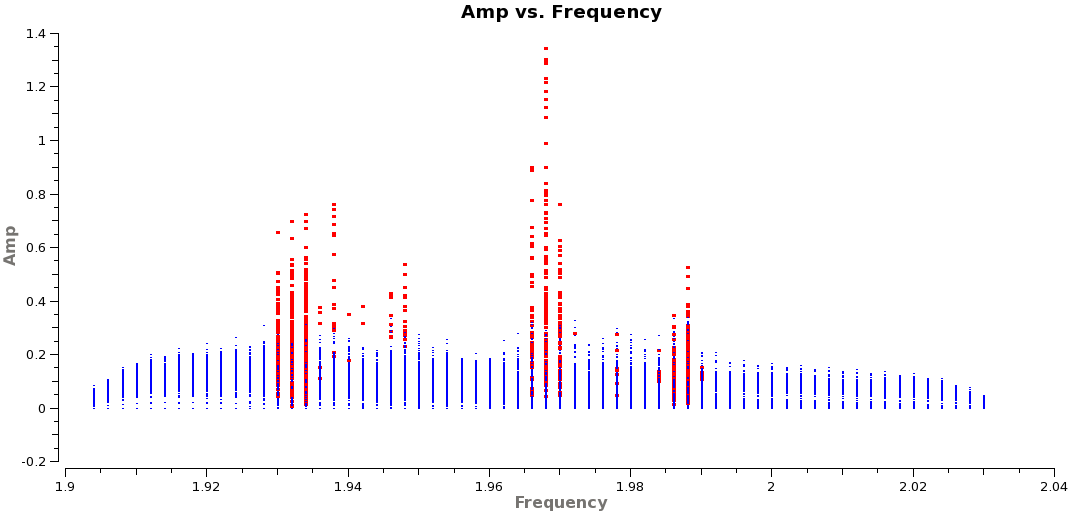
\includegraphics[scale=0.5]{plot.spectrum.ea11.spw9.1s.png}
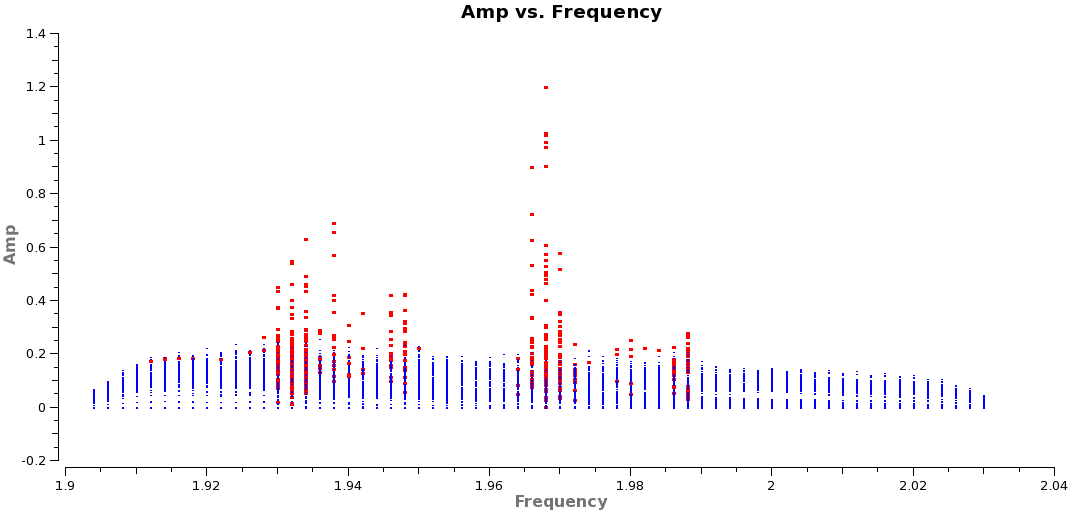
\includegraphics[scale=0.5]{plot.spectrum.ea11.spw9.avg10s.png}
\caption{Data amplitude vs frequency (flagged points are in red) for SPW=9, scan 7, and antenna EA11.  (FIRST) : Result of rflag run on 1sec timestep data, and averaged to 10s only during plotting.  (SECOND) : Result of rflag run on 10sec timestep data.}
\label{Fig:compare_6}
\end{figure}



\subsection{Comparison of autoflag methods}
What are the advantages and disadvantages ?  What types of RFI are the defaults of tfcrop and rflag optimized for ?  

\begin{figure}
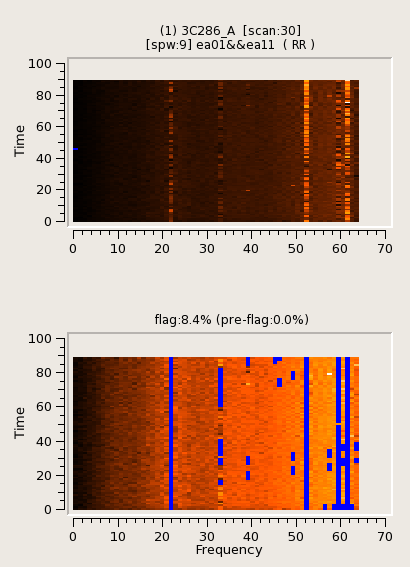
\includegraphics[scale=0.7]{rflag.before.after.png}
\caption{Example of rflag on narrow-band RFI}
\end{figure}



\subsection{Effect of Hanning-smoothing on RFI}
When does it help, when does it hurt.... 

\subsection{Is auto-flagging good-enough for imaging ?}
A comparison of images and flag-summary counts,  with only autoflag runs, and with more careful hand-flagging. 





